\documentclass[a4paper,twocolumn,10pt]{article}

\newcommand{\ignore}[1]{}
\usepackage[hyphens,spaces,obeyspaces]{url}
\usepackage{hyperref}
\usepackage{underscore}
\usepackage{multirow}
\usepackage{lastpage}
\usepackage{color}
\usepackage{caption}
\usepackage{subfig}
\usepackage{graphicx}
\usepackage{listings}
\usepackage{array}
\usepackage{paralist}
% \usepackage[title=normal,sections=normal,margins=normal,charwidths=normal,leading=normal,bibliography=normal]{savetrees}

\lstset{ %
	basicstyle=\footnotesize,
	language=C
}

% Custom paper writing commands
\newcommand{\hide}[1]{}
\newcommand{\todo}[1]{\textcolor{red}{#1}}
\newcommand{\code}[1]{\texttt{#1}}
\newcommand{\figwidth}[0]{0.95\linewidth}
\newcommand{\tblsize}[0]{\footnotesize}

\begin{document}

\pagestyle{empty}


\newcommand{\fulltitle}[0]{Paper Title}
\title{\Large \bf \fulltitle{}}

\author{
	{\rm Author 1 \hspace{.75cm}
             Author 2} \\
	Department \\
	Institution \\
	{\footnotesize \{author2,author2\}@example.com}
}

\maketitle

\begin{abstract}

Write an abstract at the end.

\end{abstract}

\section{Introduction}
\label{sec:intro}

Write a good introduction.

\begin{figure}[h]
   \centering
   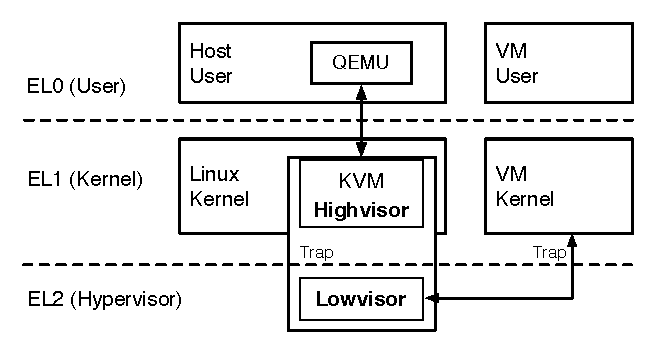
\includegraphics[width=\columnwidth{}]{figures/example}
   \caption{Example figure}\label{fig:example}
\end{figure}


% You might want to remove this as you start having citations in your
% document.  We only have this to avoid a build error from pdflatex on the
% template paper.  Of course, it's always nice to cite Popek and Goldberg.
\nocite{popekGoldberg}

\bibliographystyle{acm}

\begingroup
\raggedright
\bibliography{references}
\endgroup

\end{document}
